\section{Johdanto}
Tässä luvussa määritellään pistepilven käsite, tutustutaan laserkeilaimiin, joilla pistepilviä taltioidaan ja mainitaan muutamia yleisiä pistepilvien käsittelyn työvaiheita. Lisäksi esitellään muutama esimerkki pistepilvien käyttökohteista. Lopuksi määritellään tämän tutkielman tavoitteet, toteutustapa ja rakenne.

\subsection{Pistepilvet}

Pistepilveksi kutsutaan jotakin objektia tai maisemaa kuvaavaa suurta joukkoa pisteitä kolmiulotteisessa avaruudessa. Pistepilvi tuotetaan yleensä laserkeilaimella \engl{Laser Scanner}, joka ampuu ympärilleen laserpurskeita ja mittaa etäisyyksiä pisteisiin, joista purske heijastuu takaisin. Pistepilviä voidaan tuottaa myös synteettisesti ottamalla näytepisteitä mistä tahansa 3d-mallista, mutta tässä tutkielmassa keskitytään laserkeilaimilla tuotettuihin pistepilviin. \footnote{1980-luvulta lähtien pisteitä on ehdotettu yleisiksi renderöintiprimitiiveiksi kuvaamaan mitä tahansa geometriaa \cite{Whitted}. Ajatus on nykyään vielä ajankohtaisempi, sillä renderöitävät mallit monimutkaistuvat jatkuvasti ja usein yksittäiset polygonit projisoituvat kuvaruudulle alle pikselin kokoisina. Tällöin polygonien kärkipisteiden sijaan olisi tehokkaampaa säilyttää muistissa vain yhtä pistettä. Grafiikkakirjastot ja näytönohjaimet on kuitenkin vielä optimoitu kolmioiden käsittelyyn.}

Pistepilville on useita käyttökohteita, joista arkkitehtuuri ja rakentaminen on yksi tärkeimmistä. Pistepilvien hyödyntäminen voidaan aloittaa rakennusprojektin hyvin varhaisessa vaiheessa. Rakennettavan tontin ympäristöstä voidaan ottaa laserkeilauksia, jotta suunniteltavan rakennuksen sopimista tontille voidaan helposti arvioida. Rakennusprojektin aikana säännöllisillä laserkeilauksilla voidaan seurata tarkasti projektin etenemistä ja havaita mahdollisia ongelmia ajoissa. Pistepilvillä on myös tärkeä rooli rakennuksen valmistumisen jälkeen. Muutostöitä tehtäessä halutaan rakennuksesta saada ajantasalla oleva 3d-malli. Manuaalinen mallintaminen olisi hyvin suuri työ verrattuna muutaman kymmenen pistepilven luomiseen laserkeilaimella, mikä voidaan tehdä päivässä. \cite{bim} 

\begin{figure}
    \centering
    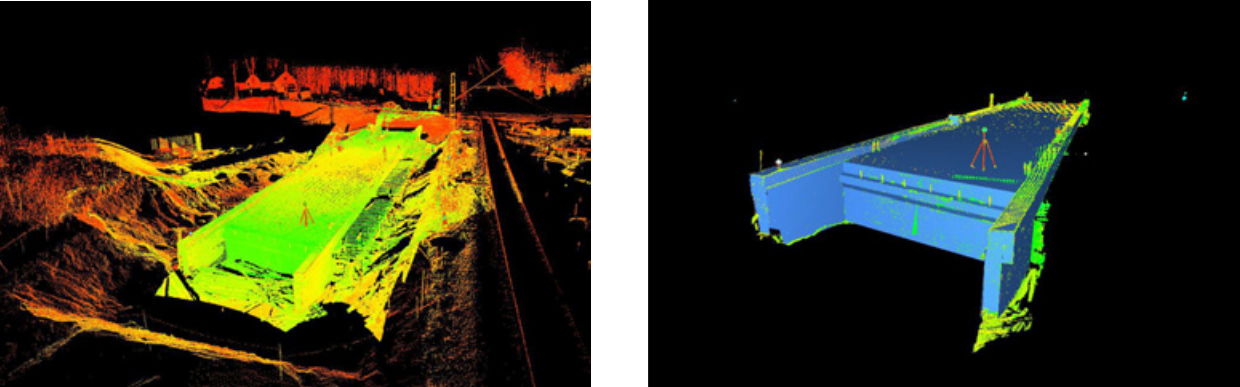
\includegraphics[width=\textwidth]{img/silta.png}
    \caption{Silta Joroisten ja Varkauden välissä Kuvasintiellä. Vasemmalla pistepilvi, oikealla pistepilvestä muodostetua geometriaa suunnitteluohjelmassa. Kuva: \cite{silta}}
    \label{silt}
\end{figure}

Eräs mielenkiintoinen sovelluuskohde laserkeilaukselle on sillanrakentaminen. Sillanrakentamisessa haasteita tuottavat tien ja maaston geometrian yhteensovittamisen lisäksi projektin pitkä kesto. Silta on rakennettava osissa ja lopputuloksen on oltava suora, minkä takia siltatyömaalla suoritetaan usein tarkistusmittauksia. Älykäs silta -projektissa tutkittiin tapoja hyödyntää tietotekniikkaa sillanrakentamisessa ja -korjaamisessa, ja havaittiin laserkeilauksen olevan hyvä tapa suorittaa tarkkuusmittauksia. Laserkeilauksella muodostettiin pistepilviä sillan kannesta ja rakenteista, jonka jälkeen niistä muodostettiin pintoja 3d-suunnitteluohjelmaan. Pistepilvi ja siitä muodostettu geometria on esitetty kuvassa \ref{silt}. \cite{silta}   

\begin{figure}
    \centering
    \includegraphics[width=0.7\paperwidth]{img/amphitheatre.png}
    \caption{Carnuntumin kaupungin amfiteatteri taltioituna laserkeilauksella. Kuva: \cite{Amphitheatre}}
    \label{amfi}
\end{figure}

Pistepilviä käytetään hyväksi myös arkeologiassa. Roomalaiset perustivat vuoden 40 tienoilla Tonavan varrelle nykyisen Itävallan alueelle
sotilasleirin, josta kasvoi myöhemmin Carnuntumin kaupunki. Kaupungin muurien ulkopuolelle rakennettiin amfiteatteri, johon mahtui 13000 katsojaa.
Vuonna 2007 Ala-Itävallan osavaltion hallitus aloitti arkeologiset kaivaukset amfiteatterin alueella, joiden yhteydessä alueesta muodostettiin kattava pistepilvi noin kahdellasadalla laserkeilauksella. Ruudunkaappaus kysesestä pistepilvestä on esitetty kuvassa \ref{amfi}. \cite{Carnuntum}

\begin{figure}
    \centering
    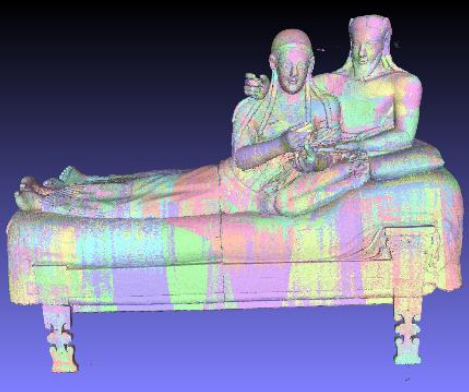
\includegraphics[width=0.4\paperwidth]{img/sarkofagi.png}
    \caption{Etruskilaisesta sarkofagista muodostettu pistepilvi. Kuva: \cite{sarkofagi}}
    \label{sarko}
\end{figure}

Pistepilviä käytetään historiallisen kulttuuriperinnön säilyttämiseen myös pienemmässä mittakaavassa. 1800-luvulla tehdyissä Cerveterin arkeologisissa kaivauksissa Italiassa löydettiin 500-luvulla terrakottasavesta tehty etruskilainen sarkofagi, joka kuvasi avioparia rentoutumassa tuonpuoleisessa. Satoihin palasiin hajonnut sarkofagi restauroitiin vuonna 1893 ja se digitoitiin käyttämällä laserkeilausta ja fotogrammetriaa vuonna 2013 taidenäyttelyä varten. Sarkofagista keilattu pistepilvi on esitetty kuvassa \ref{sarko}. \cite{sarkofagi} 

Eräs vaativa pistepilvien sovelluskohde on itseohjautuvat kulkuneuvot. Voidakseen navigoida liikenteessä itseohjautuva auto tarvitsee kameroiden ja ultraäänisensoreiden lisäksi katollen laserkeilaimen, jolla voidaan tarkkailla auton etäisyyttä muihin tienkäyttäjiin ja esteisiin. Itseohjautuvat autot ovat merkittävä tutkimuskohde myös pistepilvien käsittelyn kannalta. Auton katolle asennettavan laserkeilaimen tulisi olla tarkka, nopea ja edullinen, ja sen tuottamaa pistedataa täytyy voida käsitellä reaaliajassa. \cite{car} 

Pistepilviä voidaan käyttää myös huomattavasti suuremmassa mittakaavassa. Maanmittauslaitos on kerännyt ilmasta käsin pistepilvidataa lähes koko Suomen maaperästä. Lentokoneesta keilattu pistepilvi on melko harva - puoli pistettä neliömetriä kohden -, mutta keilattavan kohteen laajuus tekee pilvistä valtavia. Pistepilviä on käytetty lähinnä metsävarojen kartoittamiseen, mutta Maanmittauslaitos aikoo ryhtyä keräämään pistedataa tarkemmilla laserkeilamilla myös rakennuksista. \cite{hs}

\subsection{Laserkeilaimet}\label{laserkeilaimet}

Perinteinen pistepilvien mittaamiseen käytetty laserkeilain on jalustalla seisova laite, joka pyörii pystyakselinsa ympäri ampuen ympärilleen miljoonia laserpurskeita. Laserkeilain mittaa etäisyyksiä pisteisiin, joista laserpurske heijastuu takaisin keilaimeen ja muodostaa näistä pisteistä pistepilven. Heijastuksen voimakkuutta käytetään usein määräämään pisteelle väri. Yleensä tarkasteltavaa kohdetta täytyy keilata useista eri suunnista, jotta saataisiin tarpeeksi kattava joukko pistepilviä. Kohteesta riippuen voidaan tarvita jopa satoja keilauksia. Pistepilvien sovittamista yhteen tarkastellaan luvussa \ref{workflow}.

\begin{figure}
    \centering
    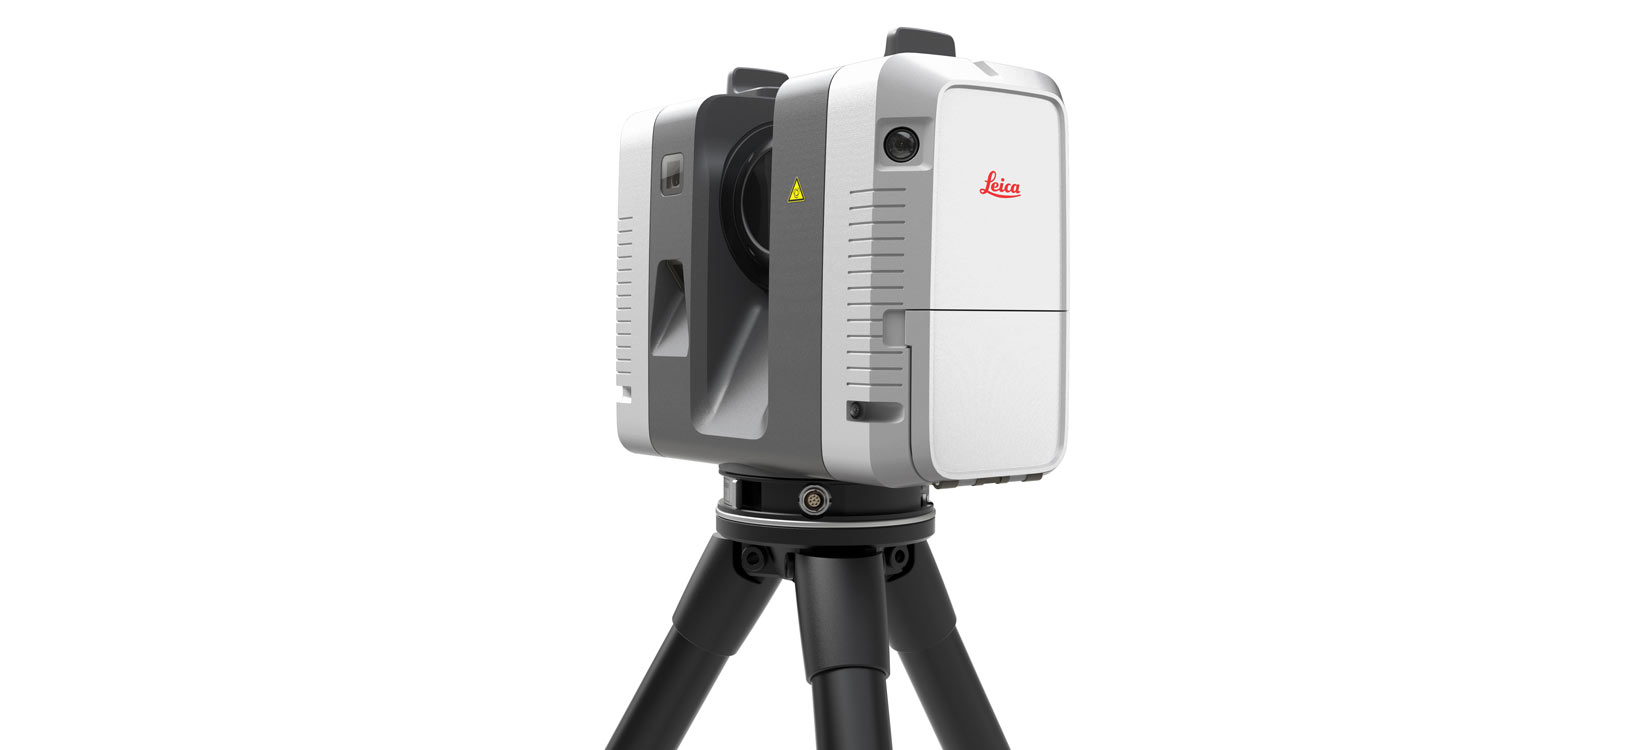
\includegraphics[width=0.7\paperwidth]{img/leica.jpg}
    \caption{Kulkuaikatekniikkaan perustuva Leica RTC360 -laserkeilain. Kuva: \url{https://leica-geosystems.com/-/media/images/leicageosystems/about-us/news\%20room/reporter/reporter-83/09-discovering-the-power-of-scanning/leica-espresso_expert_insights_640x750_slider4.ashx?la=en&hash=9D35592CBB571C3777E1E8A9A0A056BD}}
    \label{leica}
\end{figure}

Nykyaikaisella laserkeilaimella saadaan muodostettua hyvin tarkka ja tiheä pistepilvi nopeasti. Esimerkiksi kuvassa \ref{leica} näkyvä Leica Geosystemsin RTC360 -keilaimen luvataan mittaamaavan jopa kaksi miljoonaa pistettä sekunnissa ja kiertävän täyden ympyrän alle kahdessa minuutissa. Keilaimen lisäksi laitteessa on kamera, jolla saadaan määritettyä pisteille oikeat värit. \cite{leica} 

Laserkeilaimien toimintaperiaatteissa on eroja. Kaksi yleisintä toimintaperiaatetta ovat kulkuaikatekniikka \engl{Time-Of-Flight} ja vaihesiirtotekniikka \engl{phase shift}. Kulkuaikatekniikkassa pisteen etäisyys keilaimesta selviää ajasta, joka kuluu laserpurskeen lähetettämisestä sen heijastuksen vastaanottamiseen. Pisteen etäisyys keilaimesta on yksinkertaisesti 
\begin{equation}
    d=\frac{c\cdot t}{2},    
\end{equation}
missä c on valonnopeus ja t on mitattu aika. \cite{fabritius}   
Vaihesiirtotekniikka perustuu keilaimesta lähtevän signaalin vaiheen vertaamista palaavan signaalin vaiheeseen. Pisteen etäisyys keilaimesta saadaan laskemalla 
\begin{equation}
    d=n\cdot \lambda + \frac{\Phi \cdot \lambda}{2 \cdot \pi},
\end{equation}
missä n on havainnon täysien aaltojen määrä, $\lambda$ on signaalin aallonpituus ja $\Phi$ on lähtevän ja palaavan signaalin vaihe-ero. \cite{fabritius}

\begin{figure}
    \centering
    \subfile{fig/pallo.tex}
    \caption{Pallokoordinaatisto. Pisteen sijainti avaruudessa ilmaistaan korotuskulmalla $\theta$, atsimuuttikulmalla $\phi$ ja säteellä $r$.}
    \label{pallo}
\end{figure}{}

Laserkeilain tallentaa mittaamansa pisteen pallokoordinaateissa. Pisteen siirtäminen pallokoordinaateista karteesiseen koordinaatistoon onnistuu laskemalla koordinaatit 
\begin{equation}
    \begin{split}
        x&=r \cdot \sin \theta \cdot \cos \phi,\\ 
        y&=r \cdot \sin \theta \cdot \cos \phi,\\
        z&=r \cdot \cos \theta,    
    \end{split}
\end{equation}
missä r on pallon säde, $\theta$ on korotuskulma ja $\phi$ atsimuuttikulma. Pallokoordinaatistoa on havainnollistettu kuvassa \ref{pallo}.

\subsection{Pistepilvidatan käsittely}\label{workflow}

\subsubsection{Rekisteröinti}

Laserkeilauksen tuottama pistepilvi sisältää joukon pisteitä koordinaatistossa, jonka origona on keilaimen sijainti. Usein keilauksen kohteesta otetaan kymmeniä tai jopa satoja keilauksia, jotka täytyy saada samaan koordinaatistoon. Tätä kutsutaan pistepilvien rekisteröinniksi. 

Pistepilvet voidaan reksiteröidä usealla eri tavalla. Joskus keilattavaan kohteeseen asetetaan erityisiä merkkikuvioita, jotka näkyvät useasta keilaimesta. Kun tiedetään merkkien etäisyys ja suunta kustakin keilaimesta, voidaan pistepilvet sovittaa yhteen koordinaatistoon. Joissakin sovelluksissa käyttäjä merkitsee pilvistä pisteitä, jotka kuvaavat samaa aluetta.

\begin{figure}
    \begin{subfigure}{.5\textwidth}
        \centering
        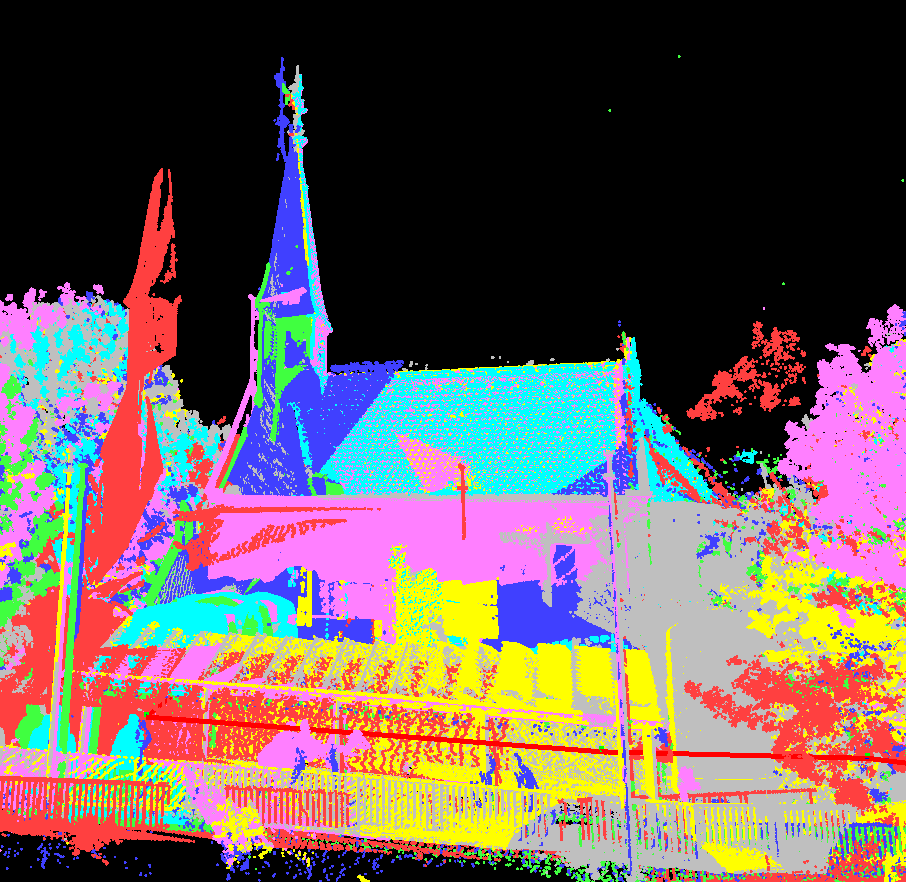
\includegraphics[width=.89\linewidth]{img/reg1.png}
        \caption{}
        %\label{fig:sub1}
    \end{subfigure}%
    \begin{subfigure}{.5\textwidth}
        \centering
        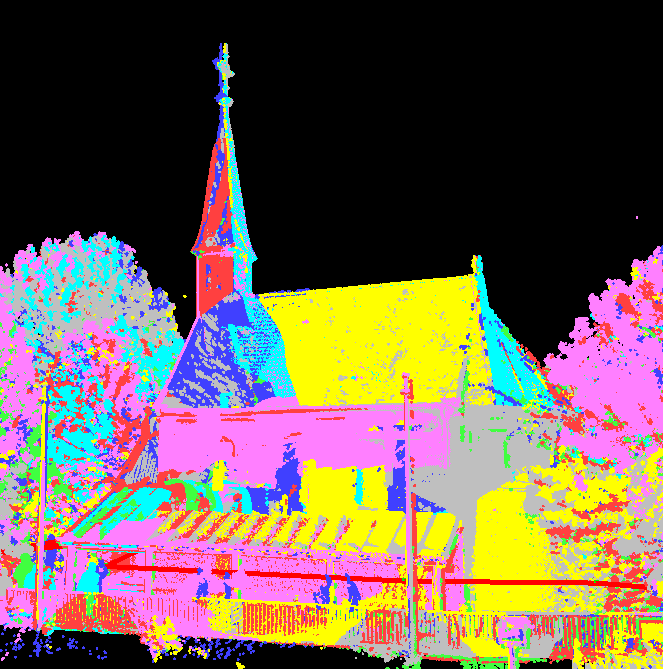
\includegraphics[width=.855\linewidth]{img/reg2.png}
        \caption{}
        %\label{fig:sub2}
    \end{subfigure}
    \caption{Saksan Würzburgissa sijaitsevasta Randersackerin Neitsyt Marian kärsimysten kappelista keilattuja pistepilviä (a) ennen rekisteröintiä ja (b) rekisteröinnin jälkeen. Kunkin keilauksen pisteet on piirretty eri väreillä.}
    \label{img:reg}
\end{figure}

Pistepilviä voidaan rekisteröidä myös ilman merkkikuvioita. Iteratiivinen lähimmän pisteen algoritmi \engl{iterative closest point, ICP} sovittaa pistepilven toiseen etsimällä rotaation ja translaation, jolla pilvien välinen virhe saadaan minimoitua. ICP-algoritmi määrittää ensin pilvistä toisiaan vastaavat pisteet ja virhe lasketaan kaikkien vastaavuuksien välisistä etäisyyksistä. Yksinkertaisimmillaan pistettä vastaavaksi pisteeksi merkitään sovitettavan pilven lähinnä sijaitseva piste. 
ICP-algoritmi tarvitsee käyttäjältä usein hyvän alkuarvauksen, jotta pilvien sovittaminen onnistuisi. 
\footnote{Täysin automaattista pistepilvien rekisteröintiä on tutkittu paljon, ks. esim. \cite{Pascal}.} Kuvassa \ref{img:reg} on ICP-algoritmilla sovitettu yhteen kuusi pistepilveä. 


\subsubsection{Muukalaispisteiden poistaminen}

Pistepilvissä on usein muukalaispisteitä \engl{outlier}, johtuen esimerkiksi laserkeilaimen epätarkkuudesta tai vaikkapa tuulen heiluttamista puiden lehdistä. Yksinkertainen tekniikka poistaa muukalaispisteitä pilvestä on verrata pisteen normaalivektoria sen naapuripisteiden normaaleihin. Pisteen $p_i$ normaalivektori voidaan selvittää pääkomponenttianalyysillä \engl{principal component analysis, PCA}. Ensin on etsittävä pilvestä pisteen $p_i$ $k$ lähintä naapuria, jonka jälkeen naapurston pisteistä lasketaan ominaisarvot. Kahta suurinta ominaisarvoa vastaavaa ominaisvektoria voidaan käyttää kuvaamaan tasoa, joka sovitetaan naapuruston päälle. Jäljelle jäävä ominaisvektori kuvaa pisteen $p_i$ normaalia. \cite{huang}

\subsubsection{Geometrian rekonstruointi}

Joissakin sovelluksissa halutaan luoda pistedatasta kohteen pintoja kuvaava polygoniverkko, jotta renderöinti olisi nopeampaa olemassaolevilla grafiikkakirjastoilla ja visuaalinen lopputulos parempi. Yksinkertainen tekniikka luoda tiivis kolmiointi pistepilvestä on Delaunayn kolmiointi\footnote{Delaunayn kolmiointi sopii harvoin oikeilla laserkeilaimilla taltioituihin, häiriötä sisältäviin pistepilviin. Hyvän yleiskatsauksen realistisemmista pinnanmuodostustekniikoista ovat julkaisseet esim. \cite{berger}} \engl{Delaunay triangulation}. Delaunayn kolmiointi perustuu Voronoin diagrammiin \engl{Voronoi diagram}, joka jakaa pisteitä sisältävän tason tai avaruuden konvekseihin Voronoin soluihin. Voronoin solu kattaa sen alueen, jossa etäisyys solua vastaavaan pisteeseen on pienempi kuin muihin pisteisiin. Kahden solun välillä on Voronoin jana, josta etäisyys kahteen pisteeseen on sama, ja kolmen janan leikkauspisteessä on Voronoin kärki, josta etäisyys kolmeen pisteeseen on yhtä suuri. Delaunayn kolmiointi on Voronoin diagrammin duaaligraafi, josta luodaan graafi siten, että pisteiden välillä on kaari, mikäli niitä vastaavat Voronoin solut jakavat Voronoin janan. \cite{delaunay}

\subsubsection{Panoramakuvat}

\begin{figure}
    \centering
    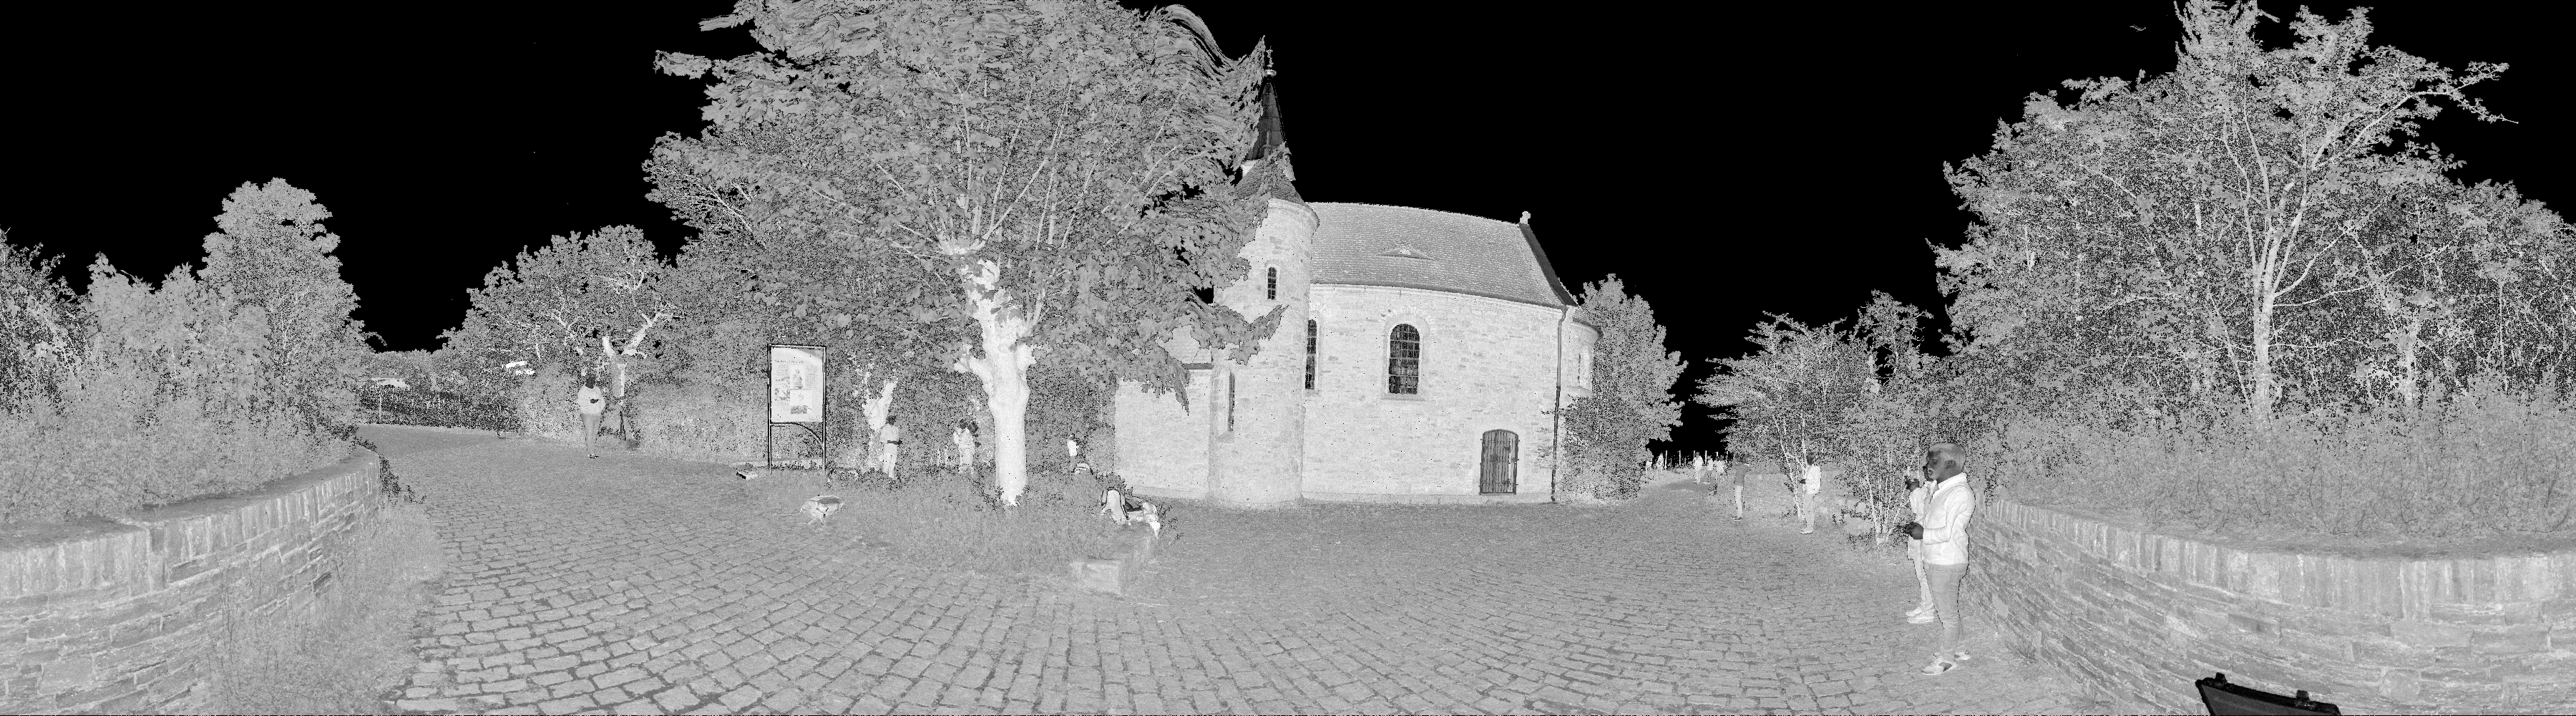
\includegraphics[width=\textwidth]{img/pano.png}
    \caption{Kuvan \ref{img:reg} kappelista keilatusta pistepilvestä luotu panoramakuva.}
    \label{img:pano}
\end{figure}


Joskus pistepilvet halutaan kompaktimpaan esitysmuotoon, jossa niiden käsittely on helpompaa. Pistepilvestä voidaan luoda panoramakuva projisoimalla laserkeilaimen ympäröimät pisteet kaksiulotteiselle kuvatasolle.\footnote{Projektio vaikuttaa suuresti panoramakuvan laatuun. Hyvän yleiskatsauksen projektiohin antaa \cite{proj}. Kuvassa \ref{img:pano} on käytetty tasavälistä lieriöprojektiota \engl{Equirectangular projection}.} Panoramakuvan resoluutiosta riippuen pistepilvestä voidaan karsia huomattava määrä pisteitä, joiden koko olisi liian pieni projisoituna kuvatasolle. Panoramakuvaan on helppo soveltaa erilaisia kuvankäsittelyalgoritmeja, kuten piirteentunnistusta \engl{feature detection}. Kuvassa \ref{img:pano} on esimerkki panoramakuvasta.

\subsection{Pistepilvien hyödyntäminen tietokoneavusteisessa suunnittelussa}

Aiemmin mainittiin erilaisia sovelluksia laserkeilainten tuottamille pistepilville. Tässä tutkielmassa keskitytään pistepilvien hyödyntämiseen tietokoneavusteisessa suunnittelussa \engl{computer aided design, CAD} ja erityisesti laitossuunnitteluohjelmistoissa \engl{plant design software}.

Tietokoneavusteisessa suunnittelussa pistepilviä käytetään olemassaolevien rakenteiden taltiointiin. Usein käytetty esimerkki on autoteollisuuden alalta: ryhmä suunnittelijoita kokeilee uutta korimallia rakentamalla prototyyppiauton helposti muovattavasta materiaalista. Kun prototyyppi on todettu aerodynaamiseksi ja miellyttävän näköiseksi, täytyy se saada digitoitua, jotta se voidaan siirtää massatuotantoon. Usein yksinkertaisin ja kustannustehokkain tapa on laserkeilata prototyyppi ja jatkokäsitellä pistepilveä niin, että saadaan luotua haluttu 3d-malli.

Laitossuunnittelussa yleisempi ongelma on 3d-mallin vanhentuminen tai sen puuttuminen kokonaan. Vaikka laitosta alunperin suunniteltaessa siitä olisi tehty 3d-malli, laitteistojen sommittelua saatetaan muuttaa ilman, että samoja muutoksia tehdään 3d-malliin. Kun 3d-mallia halutaan taas hyödyntää, voi olla kustannustehokkaampaa luoda laitoksesta laserkeilaimella pistepilvi kuin mallintaa tehdyt muutokset suunnitteluohjelmalla. \cite{Piipponen}

Kuten sillanrakennuksessa, myös laitoksia rakentaessa on joskus syytä suorittaa tarkastusmittauksia ja verrata niitä alkuperäiseen 3d-malliin. Pistepilvet ovat tähänkin tarkoitukseen sopivia. Nykyaikaisten laserkeilainten tuottamat pistepilvet ovat niin tarkkoja, että niistä voi havaita esimerkiksi putkien roikkumisen ja lämpölaajenemisen \cite{Piipponen}. 

Pistepilviä voi hyödyntää monin tavoin laitossuunnittelussa. Jos laitokseen halutaan vaikkapa uusi vesiputki, voidaan sen mahtuminen varmistaa reitittämällä putki suunnitteluohjelmistolla ja tarkastamalla, osuuko se pistepilveen. Jos taas vanhasta laitoksesta halutaan luoda ajantasalla oleva 3d-malli, voi suunnittelija mallintaa laitosta pistepilvien avulla. Pistepilven päälle on helppo sijoittaa suunnitteluohjelman putkistoja ja laitteita oikeille paikoilleen. Markkinoilla on myös ohjelmistoja, joiden luvataan tuottavan pistepilvestä automaattisesti älykäs 3d-malli komponenttitietoineen ilman aikaavievää päällemallinnusta \cite{aveva}. 

Tietokoneavusteisen suunnittelun ohjelmisto käsittelee pistepilviä eri tavoin riippuen suunnittelutyön luonteesta. Kappalemallinnuksessa visualisoidaan usein yksittäisiä osia, joita kuvaavat pistepilvet ovat hyvin tiiviitä ja usein kaikki pisteet ovat kerralla näkyvissä. Laitossuunnittelussa pistepilvet ovat taas hyvin laajoja ja voivat kuvata esimerkiksi kokonaista tehdasaluetta. Näissä sovelluksissa on tärkeää pistepilven nopea rajaaminen niin, että vain näkymän sisältävät pisteet renderöidään. Usein on tarpeen myös käyttää eri tarkkuuksia pistepilven eri osille; kaukana katsojasta sijaitsevista pisteistä renderöidään vain osa \cite{mikko}. Joitakin yleisiä käyttötapauksia pistepilvien kanssa työskentelystä laitossuunnittelussa ja niiden esittämiä vaatimuksia laitossuunnitteluohjelmistolle on esitetty luvussa \ref{usecase}.


\subsection{Tutkielman tavoitteet ja rakenne}

Tämän tutkielman tarkoituksena on tutustua pistepilvien käsittelyn ja visualisoinnin tuottamiin ongelmiin ja selvittää niihin ratkaisuvaihtoehtoja alan julkaisujen pohjalta. Selvitystyön pohjalta kehitetään tietorakenne erityisesti laitossuunnitteluohjelmiston tarpeisiin. Lopuksi arvioidaan tietorakenteen suorituskykyä ja soveltuvuutta tehtävään käyttäen verrokkina yksinkertaista ei-hierarkista tietorakennetta.

Tässä luvussa on perehdytty pistepilviin ja laserkeilaimiin yleisellä tasolla. Luvussa \ref{kirjallisuus} tutustutaan alan kirjallisuuteen ja esitellään tietorakenteita, joiden ominaisuuksia voisi hyödyntää myös laitossuunnitteluohjelmistossa. Luvussa \ref{mun} määritellään vaatimuksia, joita laitossuunnitteluohjelmisto asettaa pistepilvien käsittelyyn ja visualisointiin käytetylle tietorakenteelle. Tämän jälkeen ehdotetaan luvussa \ref{kirjallisuus} esiteltyihin julkaisuihin perustuva, laitossuunnitteluohjelmistoon soveltuva tietorakenne. Tätä tietorakennetta verrataan yksinkertaiseen toteutukseen luvussa \ref{arviointi}.

Tämä tutkielma on tehty CADMATIC Oy:n toimeksiantona. CADMATIC on suomalainen ohjelmistoyritys, joka kehittää tuotteita laivojen ja laitosten tietokoneavusteiseen suunnitteluun. CADMATIC on toiminut alalla 1980-luvulta lähtien ja sillä on asiakkainaan yli tuhat organisaatiota yli viidestäkymmenestä maasta \cite{cadmatic}. Yrityksen pääkonttori on Turussa. Tutkielmassa kehitettävää tietorakennetta testataan CADMATIC Plant Modeller -laitossuunnitteluohjelmistossa, sekä eBrowser-mallinkatseluohjelmistossa. 